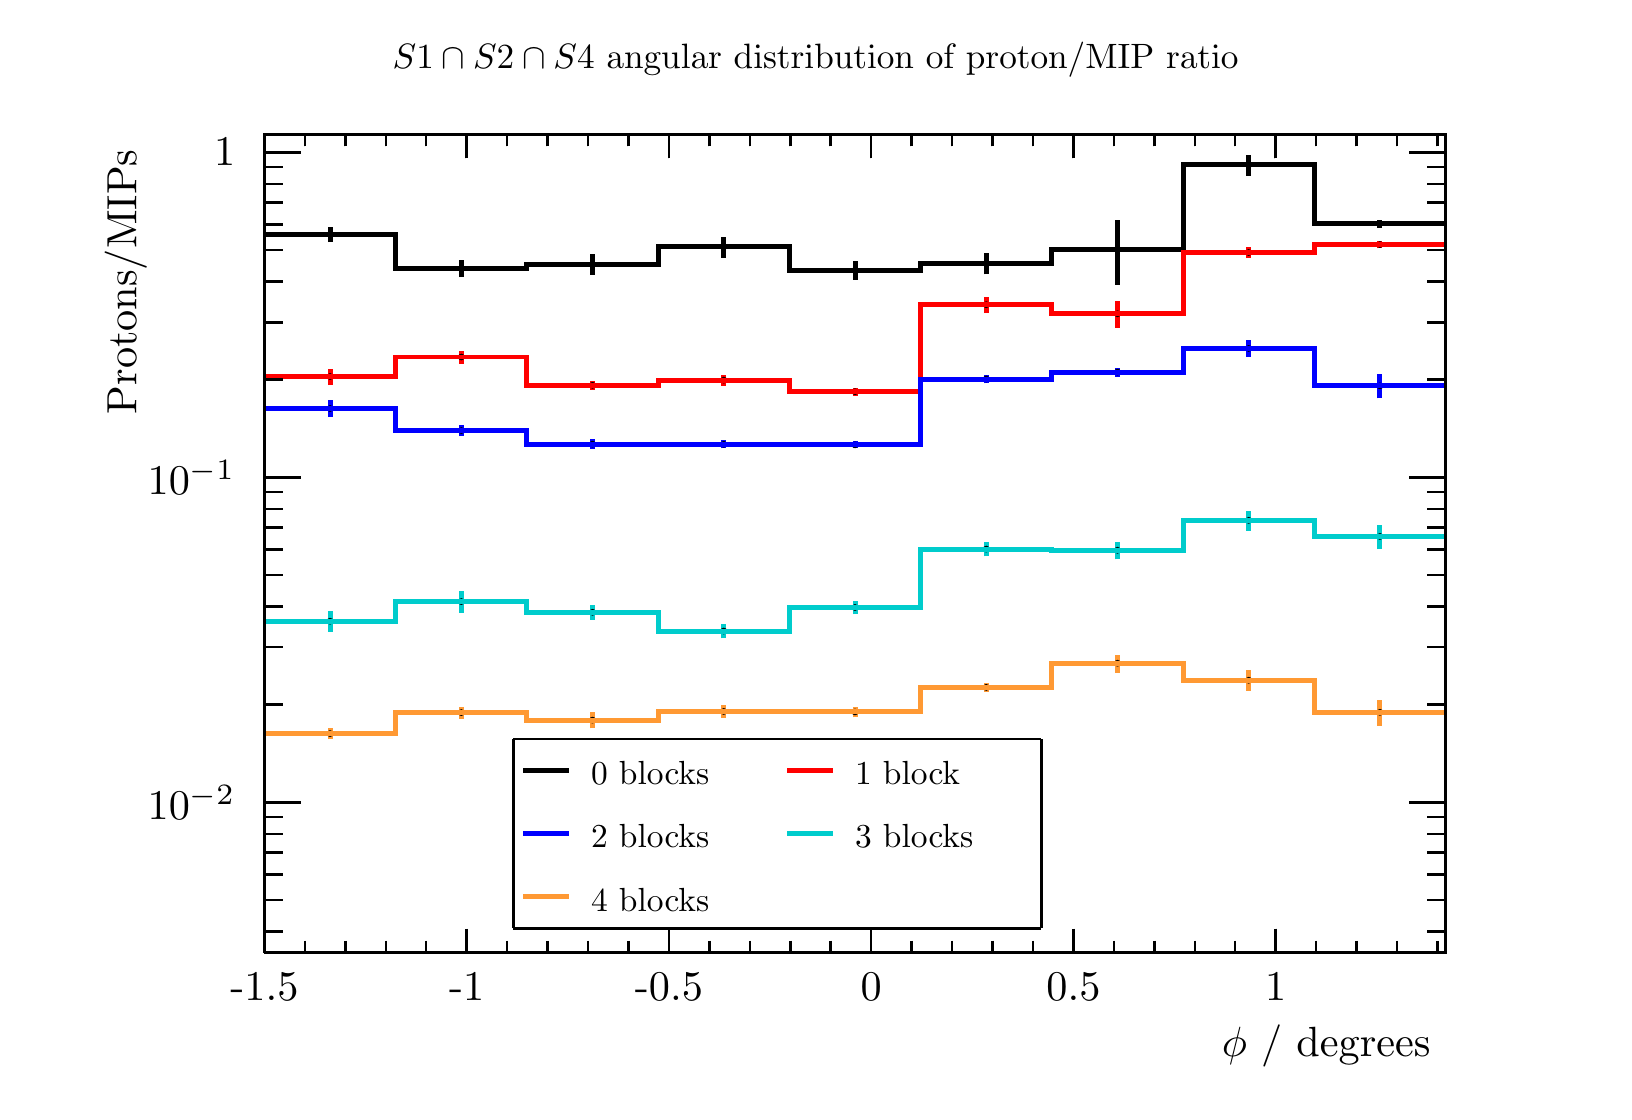
\begin{tikzpicture}
\pgfdeclareplotmark{cross} {
\pgfpathmoveto{\pgfpoint{-0.3\pgfplotmarksize}{\pgfplotmarksize}}
\pgfpathlineto{\pgfpoint{+0.3\pgfplotmarksize}{\pgfplotmarksize}}
\pgfpathlineto{\pgfpoint{+0.3\pgfplotmarksize}{0.3\pgfplotmarksize}}
\pgfpathlineto{\pgfpoint{+1\pgfplotmarksize}{0.3\pgfplotmarksize}}
\pgfpathlineto{\pgfpoint{+1\pgfplotmarksize}{-0.3\pgfplotmarksize}}
\pgfpathlineto{\pgfpoint{+0.3\pgfplotmarksize}{-0.3\pgfplotmarksize}}
\pgfpathlineto{\pgfpoint{+0.3\pgfplotmarksize}{-1.\pgfplotmarksize}}
\pgfpathlineto{\pgfpoint{-0.3\pgfplotmarksize}{-1.\pgfplotmarksize}}
\pgfpathlineto{\pgfpoint{-0.3\pgfplotmarksize}{-0.3\pgfplotmarksize}}
\pgfpathlineto{\pgfpoint{-1.\pgfplotmarksize}{-0.3\pgfplotmarksize}}
\pgfpathlineto{\pgfpoint{-1.\pgfplotmarksize}{0.3\pgfplotmarksize}}
\pgfpathlineto{\pgfpoint{-0.3\pgfplotmarksize}{0.3\pgfplotmarksize}}
\pgfpathclose
\pgfusepathqstroke
}
\pgfdeclareplotmark{cross*} {
\pgfpathmoveto{\pgfpoint{-0.3\pgfplotmarksize}{\pgfplotmarksize}}
\pgfpathlineto{\pgfpoint{+0.3\pgfplotmarksize}{\pgfplotmarksize}}
\pgfpathlineto{\pgfpoint{+0.3\pgfplotmarksize}{0.3\pgfplotmarksize}}
\pgfpathlineto{\pgfpoint{+1\pgfplotmarksize}{0.3\pgfplotmarksize}}
\pgfpathlineto{\pgfpoint{+1\pgfplotmarksize}{-0.3\pgfplotmarksize}}
\pgfpathlineto{\pgfpoint{+0.3\pgfplotmarksize}{-0.3\pgfplotmarksize}}
\pgfpathlineto{\pgfpoint{+0.3\pgfplotmarksize}{-1.\pgfplotmarksize}}
\pgfpathlineto{\pgfpoint{-0.3\pgfplotmarksize}{-1.\pgfplotmarksize}}
\pgfpathlineto{\pgfpoint{-0.3\pgfplotmarksize}{-0.3\pgfplotmarksize}}
\pgfpathlineto{\pgfpoint{-1.\pgfplotmarksize}{-0.3\pgfplotmarksize}}
\pgfpathlineto{\pgfpoint{-1.\pgfplotmarksize}{0.3\pgfplotmarksize}}
\pgfpathlineto{\pgfpoint{-0.3\pgfplotmarksize}{0.3\pgfplotmarksize}}
\pgfpathclose
\pgfusepathqfillstroke
}
\pgfdeclareplotmark{newstar} {
\pgfpathmoveto{\pgfqpoint{0pt}{\pgfplotmarksize}}
\pgfpathlineto{\pgfqpointpolar{44}{0.5\pgfplotmarksize}}
\pgfpathlineto{\pgfqpointpolar{18}{\pgfplotmarksize}}
\pgfpathlineto{\pgfqpointpolar{-20}{0.5\pgfplotmarksize}}
\pgfpathlineto{\pgfqpointpolar{-54}{\pgfplotmarksize}}
\pgfpathlineto{\pgfqpointpolar{-90}{0.5\pgfplotmarksize}}
\pgfpathlineto{\pgfqpointpolar{234}{\pgfplotmarksize}}
\pgfpathlineto{\pgfqpointpolar{198}{0.5\pgfplotmarksize}}
\pgfpathlineto{\pgfqpointpolar{162}{\pgfplotmarksize}}
\pgfpathlineto{\pgfqpointpolar{134}{0.5\pgfplotmarksize}}
\pgfpathclose
\pgfusepathqstroke
}
\pgfdeclareplotmark{newstar*} {
\pgfpathmoveto{\pgfqpoint{0pt}{\pgfplotmarksize}}
\pgfpathlineto{\pgfqpointpolar{44}{0.5\pgfplotmarksize}}
\pgfpathlineto{\pgfqpointpolar{18}{\pgfplotmarksize}}
\pgfpathlineto{\pgfqpointpolar{-20}{0.5\pgfplotmarksize}}
\pgfpathlineto{\pgfqpointpolar{-54}{\pgfplotmarksize}}
\pgfpathlineto{\pgfqpointpolar{-90}{0.5\pgfplotmarksize}}
\pgfpathlineto{\pgfqpointpolar{234}{\pgfplotmarksize}}
\pgfpathlineto{\pgfqpointpolar{198}{0.5\pgfplotmarksize}}
\pgfpathlineto{\pgfqpointpolar{162}{\pgfplotmarksize}}
\pgfpathlineto{\pgfqpointpolar{134}{0.5\pgfplotmarksize}}
\pgfpathclose
\pgfusepathqfillstroke
}
\definecolor{c}{rgb}{1,1,1};
\draw [color=c, fill=c] (0,0) rectangle (20,13.4957);
\draw [color=c, fill=c] (3,1.75444) rectangle (18,12.1461);
\definecolor{c}{rgb}{0,0,0};
\draw [c,line width=0.9] (3,1.75444) -- (3,12.1461) -- (18,12.1461) -- (18,1.75444) -- (3,1.75444);
\definecolor{c}{rgb}{1,1,1};
\draw [color=c, fill=c] (3,1.75444) rectangle (18,12.1461);
\definecolor{c}{rgb}{0,0,0};
\draw [c,line width=0.9] (3,1.75444) -- (3,12.1461) -- (18,12.1461) -- (18,1.75444) -- (3,1.75444);
\draw [c,line width=0.9] (3,1.75444) -- (4.66667,1.75444) -- (4.66667,1.75444) -- (6.33333,1.75444) -- (6.33333,1.75444) -- (8,1.75444) -- (8,1.75444) -- (9.66667,1.75444) -- (9.66667,1.75444) -- (11.3333,1.75444) -- (11.3333,1.75444) -- (13,1.75444)
 -- (13,1.75444) -- (14.6667,1.75444) -- (14.6667,1.75444) -- (16.3333,1.75444) -- (16.3333,1.75444) -- (18,1.75444);
\draw [c,line width=0.9] (3,1.75444) -- (18,1.75444);
\draw [c,line width=0.9] (3,2.05809) -- (3,1.75444);
\draw [c,line width=0.9] (3.5137,1.90627) -- (3.5137,1.75444);
\draw [c,line width=0.9] (4.0274,1.90627) -- (4.0274,1.75444);
\draw [c,line width=0.9] (4.5411,1.90627) -- (4.5411,1.75444);
\draw [c,line width=0.9] (5.05479,1.90627) -- (5.05479,1.75444);
\draw [c,line width=0.9] (5.56849,2.05809) -- (5.56849,1.75444);
\draw [c,line width=0.9] (6.08219,1.90627) -- (6.08219,1.75444);
\draw [c,line width=0.9] (6.59589,1.90627) -- (6.59589,1.75444);
\draw [c,line width=0.9] (7.10959,1.90627) -- (7.10959,1.75444);
\draw [c,line width=0.9] (7.62329,1.90627) -- (7.62329,1.75444);
\draw [c,line width=0.9] (8.13699,2.05809) -- (8.13699,1.75444);
\draw [c,line width=0.9] (8.65069,1.90627) -- (8.65069,1.75444);
\draw [c,line width=0.9] (9.16438,1.90627) -- (9.16438,1.75444);
\draw [c,line width=0.9] (9.67808,1.90627) -- (9.67808,1.75444);
\draw [c,line width=0.9] (10.1918,1.90627) -- (10.1918,1.75444);
\draw [c,line width=0.9] (10.7055,2.05809) -- (10.7055,1.75444);
\draw [c,line width=0.9] (11.2192,1.90627) -- (11.2192,1.75444);
\draw [c,line width=0.9] (11.7329,1.90627) -- (11.7329,1.75444);
\draw [c,line width=0.9] (12.2466,1.90627) -- (12.2466,1.75444);
\draw [c,line width=0.9] (12.7603,1.90627) -- (12.7603,1.75444);
\draw [c,line width=0.9] (13.274,2.05809) -- (13.274,1.75444);
\draw [c,line width=0.9] (13.7877,1.90627) -- (13.7877,1.75444);
\draw [c,line width=0.9] (14.3014,1.90627) -- (14.3014,1.75444);
\draw [c,line width=0.9] (14.8151,1.90627) -- (14.8151,1.75444);
\draw [c,line width=0.9] (15.3288,1.90627) -- (15.3288,1.75444);
\draw [c,line width=0.9] (15.8425,2.05809) -- (15.8425,1.75444);
\draw [c,line width=0.9] (15.8425,2.05809) -- (15.8425,1.75444);
\draw [c,line width=0.9] (16.3562,1.90627) -- (16.3562,1.75444);
\draw [c,line width=0.9] (16.8699,1.90627) -- (16.8699,1.75444);
\draw [c,line width=0.9] (17.3836,1.90627) -- (17.3836,1.75444);
\draw [c,line width=0.9] (17.8973,1.90627) -- (17.8973,1.75444);
\draw [anchor=base] (3,1.14713) node[scale=1.52731, color=c, rotate=0]{-1.5};
\draw [anchor=base] (5.56849,1.14713) node[scale=1.52731, color=c, rotate=0]{-1};
\draw [anchor=base] (8.13699,1.14713) node[scale=1.52731, color=c, rotate=0]{-0.5};
\draw [anchor=base] (10.7055,1.14713) node[scale=1.52731, color=c, rotate=0]{0};
\draw [anchor=base] (13.274,1.14713) node[scale=1.52731, color=c, rotate=0]{0.5};
\draw [anchor=base] (15.8425,1.14713) node[scale=1.52731, color=c, rotate=0]{1};
\draw [anchor= east] (18,0.566819) node[scale=1.52731, color=c, rotate=0]{$\phi$ / degrees};
\draw [c,line width=0.9] (3,12.1461) -- (18,12.1461);
\draw [c,line width=0.9] (3,11.8425) -- (3,12.1461);
\draw [c,line width=0.9] (3.5137,11.9943) -- (3.5137,12.1461);
\draw [c,line width=0.9] (4.0274,11.9943) -- (4.0274,12.1461);
\draw [c,line width=0.9] (4.5411,11.9943) -- (4.5411,12.1461);
\draw [c,line width=0.9] (5.05479,11.9943) -- (5.05479,12.1461);
\draw [c,line width=0.9] (5.56849,11.8425) -- (5.56849,12.1461);
\draw [c,line width=0.9] (6.08219,11.9943) -- (6.08219,12.1461);
\draw [c,line width=0.9] (6.59589,11.9943) -- (6.59589,12.1461);
\draw [c,line width=0.9] (7.10959,11.9943) -- (7.10959,12.1461);
\draw [c,line width=0.9] (7.62329,11.9943) -- (7.62329,12.1461);
\draw [c,line width=0.9] (8.13699,11.8425) -- (8.13699,12.1461);
\draw [c,line width=0.9] (8.65069,11.9943) -- (8.65069,12.1461);
\draw [c,line width=0.9] (9.16438,11.9943) -- (9.16438,12.1461);
\draw [c,line width=0.9] (9.67808,11.9943) -- (9.67808,12.1461);
\draw [c,line width=0.9] (10.1918,11.9943) -- (10.1918,12.1461);
\draw [c,line width=0.9] (10.7055,11.8425) -- (10.7055,12.1461);
\draw [c,line width=0.9] (11.2192,11.9943) -- (11.2192,12.1461);
\draw [c,line width=0.9] (11.7329,11.9943) -- (11.7329,12.1461);
\draw [c,line width=0.9] (12.2466,11.9943) -- (12.2466,12.1461);
\draw [c,line width=0.9] (12.7603,11.9943) -- (12.7603,12.1461);
\draw [c,line width=0.9] (13.274,11.8425) -- (13.274,12.1461);
\draw [c,line width=0.9] (13.7877,11.9943) -- (13.7877,12.1461);
\draw [c,line width=0.9] (14.3014,11.9943) -- (14.3014,12.1461);
\draw [c,line width=0.9] (14.8151,11.9943) -- (14.8151,12.1461);
\draw [c,line width=0.9] (15.3288,11.9943) -- (15.3288,12.1461);
\draw [c,line width=0.9] (15.8425,11.8425) -- (15.8425,12.1461);
\draw [c,line width=0.9] (15.8425,11.8425) -- (15.8425,12.1461);
\draw [c,line width=0.9] (16.3562,11.9943) -- (16.3562,12.1461);
\draw [c,line width=0.9] (16.8699,11.9943) -- (16.8699,12.1461);
\draw [c,line width=0.9] (17.3836,11.9943) -- (17.3836,12.1461);
\draw [c,line width=0.9] (17.8973,11.9943) -- (17.8973,12.1461);
\draw [c,line width=0.9] (3,1.75444) -- (3,12.1461);
\draw [c,line width=0.9] (3.231,2.0228) -- (3,2.0228);
\draw [c,line width=0.9] (3.231,2.42276) -- (3,2.42276);
\draw [c,line width=0.9] (3.231,2.74954) -- (3,2.74954);
\draw [c,line width=0.9] (3.231,3.02584) -- (3,3.02584);
\draw [c,line width=0.9] (3.231,3.26518) -- (3,3.26518);
\draw [c,line width=0.9] (3.231,3.47629) -- (3,3.47629);
\draw [c,line width=0.9] (3.462,3.66514) -- (3,3.66514);
\draw [anchor= east] (2.82,3.66514) node[scale=1.52731, color=c, rotate=0]{$10^{-2}$};
\draw [c,line width=0.9] (3.231,4.90752) -- (3,4.90752);
\draw [c,line width=0.9] (3.231,5.63427) -- (3,5.63427);
\draw [c,line width=0.9] (3.231,6.1499) -- (3,6.1499);
\draw [c,line width=0.9] (3.231,6.54986) -- (3,6.54986);
\draw [c,line width=0.9] (3.231,6.87665) -- (3,6.87665);
\draw [c,line width=0.9] (3.231,7.15295) -- (3,7.15295);
\draw [c,line width=0.9] (3.231,7.39229) -- (3,7.39229);
\draw [c,line width=0.9] (3.231,7.6034) -- (3,7.6034);
\draw [c,line width=0.9] (3.462,7.79224) -- (3,7.79224);
\draw [anchor= east] (2.82,7.79224) node[scale=1.52731, color=c, rotate=0]{$10^{-1}$};
\draw [c,line width=0.9] (3.231,9.03463) -- (3,9.03463);
\draw [c,line width=0.9] (3.231,9.76137) -- (3,9.76137);
\draw [c,line width=0.9] (3.231,10.277) -- (3,10.277);
\draw [c,line width=0.9] (3.231,10.677) -- (3,10.677);
\draw [c,line width=0.9] (3.231,11.0038) -- (3,11.0038);
\draw [c,line width=0.9] (3.231,11.2801) -- (3,11.2801);
\draw [c,line width=0.9] (3.231,11.5194) -- (3,11.5194);
\draw [c,line width=0.9] (3.231,11.7305) -- (3,11.7305);
\draw [c,line width=0.9] (3.462,11.9193) -- (3,11.9193);
\draw [anchor= east] (2.82,11.9193) node[scale=1.52731, color=c, rotate=0]{1};
\draw [anchor= east] (1.24,12.1461) node[scale=1.52731, color=c, rotate=90]{ Protons/MIPs};
\draw [c,line width=0.9] (18,1.75444) -- (18,12.1461);
\draw [c,line width=0.9] (17.769,2.0228) -- (18,2.0228);
\draw [c,line width=0.9] (17.769,2.42276) -- (18,2.42276);
\draw [c,line width=0.9] (17.769,2.74954) -- (18,2.74954);
\draw [c,line width=0.9] (17.769,3.02584) -- (18,3.02584);
\draw [c,line width=0.9] (17.769,3.26518) -- (18,3.26518);
\draw [c,line width=0.9] (17.769,3.47629) -- (18,3.47629);
\draw [c,line width=0.9] (17.538,3.66514) -- (18,3.66514);
\draw [c,line width=0.9] (17.769,4.90752) -- (18,4.90752);
\draw [c,line width=0.9] (17.769,5.63427) -- (18,5.63427);
\draw [c,line width=0.9] (17.769,6.1499) -- (18,6.1499);
\draw [c,line width=0.9] (17.769,6.54986) -- (18,6.54986);
\draw [c,line width=0.9] (17.769,6.87665) -- (18,6.87665);
\draw [c,line width=0.9] (17.769,7.15295) -- (18,7.15295);
\draw [c,line width=0.9] (17.769,7.39229) -- (18,7.39229);
\draw [c,line width=0.9] (17.769,7.6034) -- (18,7.6034);
\draw [c,line width=0.9] (17.538,7.79224) -- (18,7.79224);
\draw [c,line width=0.9] (17.769,9.03463) -- (18,9.03463);
\draw [c,line width=0.9] (17.769,9.76137) -- (18,9.76137);
\draw [c,line width=0.9] (17.769,10.277) -- (18,10.277);
\draw [c,line width=0.9] (17.769,10.677) -- (18,10.677);
\draw [c,line width=0.9] (17.769,11.0038) -- (18,11.0038);
\draw [c,line width=0.9] (17.769,11.2801) -- (18,11.2801);
\draw [c,line width=0.9] (17.769,11.5194) -- (18,11.5194);
\draw [c,line width=0.9] (17.769,11.7305) -- (18,11.7305);
\draw [c,line width=0.9] (17.538,11.9193) -- (18,11.9193);
\draw [c,line width=1.8] (3.83333,10.7777) -- (3.83333,10.8765);
\draw [c,line width=1.8] (3.83333,10.8765) -- (3.83333,10.9702);
\foreach \P in {(3.83333,10.8765)}{\draw[mark options={color=c,fill=c},mark size=2.402402pt,mark=*,mark size=1pt] plot coordinates {\P};}
\draw [c,line width=1.8] (5.5,10.3339) -- (5.5,10.4447);
\draw [c,line width=1.8] (5.5,10.4447) -- (5.5,10.549);
\foreach \P in {(5.5,10.4447)}{\draw[mark options={color=c,fill=c},mark size=2.402402pt,mark=*,mark size=1pt] plot coordinates {\P};}
\draw [c,line width=1.8] (7.16667,10.362) -- (7.16667,10.4971);
\draw [c,line width=1.8] (7.16667,10.4971) -- (7.16667,10.6227);
\foreach \P in {(7.16667,10.4971)}{\draw[mark options={color=c,fill=c},mark size=2.402402pt,mark=*,mark size=1pt] plot coordinates {\P};}
\draw [c,line width=1.8] (8.83333,10.5803) -- (8.83333,10.72);
\draw [c,line width=1.8] (8.83333,10.72) -- (8.83333,10.8497);
\foreach \P in {(8.83333,10.72)}{\draw[mark options={color=c,fill=c},mark size=2.402402pt,mark=*,mark size=1pt] plot coordinates {\P};}
\draw [c,line width=1.8] (10.5,10.2982) -- (10.5,10.4208);
\draw [c,line width=1.8] (10.5,10.4208) -- (10.5,10.5355);
\foreach \P in {(10.5,10.4208)}{\draw[mark options={color=c,fill=c},mark size=2.402402pt,mark=*,mark size=1pt] plot coordinates {\P};}
\draw [c,line width=1.8] (12.1667,10.371) -- (12.1667,10.5085);
\draw [c,line width=1.8] (12.1667,10.5085) -- (12.1667,10.6363);
\foreach \P in {(12.1667,10.5085)}{\draw[mark options={color=c,fill=c},mark size=2.402402pt,mark=*,mark size=1pt] plot coordinates {\P};}
\draw [c,line width=1.8] (13.8333,10.2369) -- (13.8333,10.6916);
\draw [c,line width=1.8] (13.8333,10.6916) -- (13.8333,11.054);
\foreach \P in {(13.8333,10.6916)}{\draw[mark options={color=c,fill=c},mark size=2.402402pt,mark=*,mark size=1pt] plot coordinates {\P};}
\draw [c,line width=1.8] (15.5,11.6218) -- (15.5,11.7605);
\draw [c,line width=1.8] (15.5,11.7605) -- (15.5,11.8893);
\foreach \P in {(15.5,11.7605)}{\draw[mark options={color=c,fill=c},mark size=2.402402pt,mark=*,mark size=1pt] plot coordinates {\P};}
\draw [c,line width=1.8] (17.1667,10.9639) -- (17.1667,11.0149);
\draw [c,line width=1.8] (17.1667,11.0149) -- (17.1667,11.0645);
\foreach \P in {(17.1667,11.0149)}{\draw[mark options={color=c,fill=c},mark size=2.402402pt,mark=*,mark size=1pt] plot coordinates {\P};}
\draw [c,line width=1.8] (3,10.8765) -- (4.66667,10.8765) -- (4.66667,10.4447) -- (6.33333,10.4447) -- (6.33333,10.4971) -- (8,10.4971) -- (8,10.72) -- (9.66667,10.72) -- (9.66667,10.4208) -- (11.3333,10.4208) -- (11.3333,10.5085) -- (13,10.5085) --
 (13,10.6916) -- (14.6667,10.6916) -- (14.6667,11.7605) -- (16.3333,11.7605) -- (16.3333,11.0149) -- (18,11.0149);
\definecolor{c}{rgb}{1,0,0};
\draw [c,line width=1.8] (3.83333,8.96432) -- (3.83333,9.07217);
\draw [c,line width=1.8] (3.83333,9.07217) -- (3.83333,9.17389);
\definecolor{c}{rgb}{0,0,0};
\foreach \P in {(3.83333,9.07217)}{\draw[mark options={color=c,fill=c},mark size=2.402402pt,mark=*,mark size=1pt] plot coordinates {\P};}
\definecolor{c}{rgb}{1,0,0};
\draw [c,line width=1.8] (5.5,9.23726) -- (5.5,9.32023);
\draw [c,line width=1.8] (5.5,9.32023) -- (5.5,9.39953);
\definecolor{c}{rgb}{0,0,0};
\foreach \P in {(5.5,9.32023)}{\draw[mark options={color=c,fill=c},mark size=2.402402pt,mark=*,mark size=1pt] plot coordinates {\P};}
\definecolor{c}{rgb}{1,0,0};
\draw [c,line width=1.8] (7.16667,8.90343) -- (7.16667,8.96069);
\draw [c,line width=1.8] (7.16667,8.96069) -- (7.16667,9.01617);
\definecolor{c}{rgb}{0,0,0};
\foreach \P in {(7.16667,8.96069)}{\draw[mark options={color=c,fill=c},mark size=2.402402pt,mark=*,mark size=1pt] plot coordinates {\P};}
\definecolor{c}{rgb}{1,0,0};
\draw [c,line width=1.8] (8.83333,8.95669) -- (8.83333,9.02674);
\draw [c,line width=1.8] (8.83333,9.02674) -- (8.83333,9.09415);
\definecolor{c}{rgb}{0,0,0};
\foreach \P in {(8.83333,9.02674)}{\draw[mark options={color=c,fill=c},mark size=2.402402pt,mark=*,mark size=1pt] plot coordinates {\P};}
\definecolor{c}{rgb}{1,0,0};
\draw [c,line width=1.8] (10.5,8.82806) -- (10.5,8.87953);
\draw [c,line width=1.8] (10.5,8.87953) -- (10.5,8.92957);
\definecolor{c}{rgb}{0,0,0};
\foreach \P in {(10.5,8.87953)}{\draw[mark options={color=c,fill=c},mark size=2.402402pt,mark=*,mark size=1pt] plot coordinates {\P};}
\definecolor{c}{rgb}{1,0,0};
\draw [c,line width=1.8] (12.1667,9.87581) -- (12.1667,9.98442);
\draw [c,line width=1.8] (12.1667,9.98442) -- (12.1667,10.0868);
\definecolor{c}{rgb}{0,0,0};
\foreach \P in {(12.1667,9.98442)}{\draw[mark options={color=c,fill=c},mark size=2.402402pt,mark=*,mark size=1pt] plot coordinates {\P};}
\definecolor{c}{rgb}{1,0,0};
\draw [c,line width=1.8] (13.8333,9.69229) -- (13.8333,9.86902);
\draw [c,line width=1.8] (13.8333,9.86902) -- (13.8333,10.0299);
\definecolor{c}{rgb}{0,0,0};
\foreach \P in {(13.8333,9.86902)}{\draw[mark options={color=c,fill=c},mark size=2.402402pt,mark=*,mark size=1pt] plot coordinates {\P};}
\definecolor{c}{rgb}{1,0,0};
\draw [c,line width=1.8] (15.5,10.576) -- (15.5,10.6472);
\draw [c,line width=1.8] (15.5,10.6472) -- (15.5,10.7157);
\definecolor{c}{rgb}{0,0,0};
\foreach \P in {(15.5,10.6472)}{\draw[mark options={color=c,fill=c},mark size=2.402402pt,mark=*,mark size=1pt] plot coordinates {\P};}
\definecolor{c}{rgb}{1,0,0};
\draw [c,line width=1.8] (17.1667,10.6997) -- (17.1667,10.7481);
\draw [c,line width=1.8] (17.1667,10.7481) -- (17.1667,10.7953);
\definecolor{c}{rgb}{0,0,0};
\foreach \P in {(17.1667,10.7481)}{\draw[mark options={color=c,fill=c},mark size=2.402402pt,mark=*,mark size=1pt] plot coordinates {\P};}
\definecolor{c}{rgb}{1,0,0};
\draw [c,line width=1.8] (3,9.07217) -- (4.66667,9.07217) -- (4.66667,9.32023) -- (6.33333,9.32023) -- (6.33333,8.96069) -- (8,8.96069) -- (8,9.02674) -- (9.66667,9.02674) -- (9.66667,8.87953) -- (11.3333,8.87953) -- (11.3333,9.98442) -- (13,9.98442)
 -- (13,9.86902) -- (14.6667,9.86902) -- (14.6667,10.6472) -- (16.3333,10.6472) -- (16.3333,10.7481) -- (18,10.7481);
\definecolor{c}{rgb}{0,0,1};
\draw [c,line width=1.8] (3.83333,8.55718) -- (3.83333,8.66636);
\draw [c,line width=1.8] (3.83333,8.66636) -- (3.83333,8.76928);
\definecolor{c}{rgb}{0,0,0};
\foreach \P in {(3.83333,8.66636)}{\draw[mark options={color=c,fill=c},mark size=2.402402pt,mark=*,mark size=1pt] plot coordinates {\P};}
\definecolor{c}{rgb}{0,0,1};
\draw [c,line width=1.8] (5.5,8.31557) -- (5.5,8.38631);
\draw [c,line width=1.8] (5.5,8.38631) -- (5.5,8.45436);
\definecolor{c}{rgb}{0,0,0};
\foreach \P in {(5.5,8.38631)}{\draw[mark options={color=c,fill=c},mark size=2.402402pt,mark=*,mark size=1pt] plot coordinates {\P};}
\definecolor{c}{rgb}{0,0,1};
\draw [c,line width=1.8] (7.16667,8.15197) -- (7.16667,8.21352);
\draw [c,line width=1.8] (7.16667,8.21352) -- (7.16667,8.27302);
\definecolor{c}{rgb}{0,0,0};
\foreach \P in {(7.16667,8.21352)}{\draw[mark options={color=c,fill=c},mark size=2.402402pt,mark=*,mark size=1pt] plot coordinates {\P};}
\definecolor{c}{rgb}{0,0,1};
\draw [c,line width=1.8] (8.83333,8.15946) -- (8.83333,8.21131);
\draw [c,line width=1.8] (8.83333,8.21131) -- (8.83333,8.26171);
\definecolor{c}{rgb}{0,0,0};
\foreach \P in {(8.83333,8.21131)}{\draw[mark options={color=c,fill=c},mark size=2.402402pt,mark=*,mark size=1pt] plot coordinates {\P};}
\definecolor{c}{rgb}{0,0,1};
\draw [c,line width=1.8] (10.5,8.15949) -- (10.5,8.20403);
\draw [c,line width=1.8] (10.5,8.20403) -- (10.5,8.24749);
\definecolor{c}{rgb}{0,0,0};
\foreach \P in {(10.5,8.20403)}{\draw[mark options={color=c,fill=c},mark size=2.402402pt,mark=*,mark size=1pt] plot coordinates {\P};}
\definecolor{c}{rgb}{0,0,1};
\draw [c,line width=1.8] (12.1667,8.98631) -- (12.1667,9.04063);
\draw [c,line width=1.8] (12.1667,9.04063) -- (12.1667,9.09336);
\definecolor{c}{rgb}{0,0,0};
\foreach \P in {(12.1667,9.04063)}{\draw[mark options={color=c,fill=c},mark size=2.402402pt,mark=*,mark size=1pt] plot coordinates {\P};}
\definecolor{c}{rgb}{0,0,1};
\draw [c,line width=1.8] (13.8333,9.07201) -- (13.8333,9.12799);
\draw [c,line width=1.8] (13.8333,9.12799) -- (13.8333,9.18227);
\definecolor{c}{rgb}{0,0,0};
\foreach \P in {(13.8333,9.12799)}{\draw[mark options={color=c,fill=c},mark size=2.402402pt,mark=*,mark size=1pt] plot coordinates {\P};}
\definecolor{c}{rgb}{0,0,1};
\draw [c,line width=1.8] (15.5,9.32044) -- (15.5,9.42921);
\draw [c,line width=1.8] (15.5,9.42921) -- (15.5,9.53176);
\definecolor{c}{rgb}{0,0,0};
\foreach \P in {(15.5,9.42921)}{\draw[mark options={color=c,fill=c},mark size=2.402402pt,mark=*,mark size=1pt] plot coordinates {\P};}
\definecolor{c}{rgb}{0,0,1};
\draw [c,line width=1.8] (17.1667,8.79549) -- (17.1667,8.95348);
\draw [c,line width=1.8] (17.1667,8.95348) -- (17.1667,9.09867);
\definecolor{c}{rgb}{0,0,0};
\foreach \P in {(17.1667,8.95348)}{\draw[mark options={color=c,fill=c},mark size=2.402402pt,mark=*,mark size=1pt] plot coordinates {\P};}
\definecolor{c}{rgb}{0,0,1};
\draw [c,line width=1.8] (3,8.66636) -- (4.66667,8.66636) -- (4.66667,8.38631) -- (6.33333,8.38631) -- (6.33333,8.21352) -- (8,8.21352) -- (8,8.21131) -- (9.66667,8.21131) -- (9.66667,8.20403) -- (11.3333,8.20403) -- (11.3333,9.04063) -- (13,9.04063)
 -- (13,9.12799) -- (14.6667,9.12799) -- (14.6667,9.42921) -- (16.3333,9.42921) -- (16.3333,8.95348) -- (18,8.95348);
\definecolor{c}{rgb}{0,0.8,0.8};
\draw [c,line width=1.8] (3.83333,5.82959) -- (3.83333,5.9648);
\draw [c,line width=1.8] (3.83333,5.9648) -- (3.83333,6.09053);
\definecolor{c}{rgb}{0,0,0};
\foreach \P in {(3.83333,5.9648)}{\draw[mark options={color=c,fill=c},mark size=2.402402pt,mark=*,mark size=1pt] plot coordinates {\P};}
\definecolor{c}{rgb}{0,0.8,0.8};
\draw [c,line width=1.8] (5.5,6.07356) -- (5.5,6.21409);
\draw [c,line width=1.8] (5.5,6.21409) -- (5.5,6.3444);
\definecolor{c}{rgb}{0,0,0};
\foreach \P in {(5.5,6.21409)}{\draw[mark options={color=c,fill=c},mark size=2.402402pt,mark=*,mark size=1pt] plot coordinates {\P};}
\definecolor{c}{rgb}{0,0.8,0.8};
\draw [c,line width=1.8] (7.16667,5.98519) -- (7.16667,6.07802);
\draw [c,line width=1.8] (7.16667,6.07802) -- (7.16667,6.16629);
\definecolor{c}{rgb}{0,0,0};
\foreach \P in {(7.16667,6.07802)}{\draw[mark options={color=c,fill=c},mark size=2.402402pt,mark=*,mark size=1pt] plot coordinates {\P};}
\definecolor{c}{rgb}{0,0.8,0.8};
\draw [c,line width=1.8] (8.83333,5.7463) -- (8.83333,5.84009);
\draw [c,line width=1.8] (8.83333,5.84009) -- (8.83333,5.92921);
\definecolor{c}{rgb}{0,0,0};
\foreach \P in {(8.83333,5.84009)}{\draw[mark options={color=c,fill=c},mark size=2.402402pt,mark=*,mark size=1pt] plot coordinates {\P};}
\definecolor{c}{rgb}{0,0.8,0.8};
\draw [c,line width=1.8] (10.5,6.05372) -- (10.5,6.13878);
\draw [c,line width=1.8] (10.5,6.13878) -- (10.5,6.21999);
\definecolor{c}{rgb}{0,0,0};
\foreach \P in {(10.5,6.13878)}{\draw[mark options={color=c,fill=c},mark size=2.402402pt,mark=*,mark size=1pt] plot coordinates {\P};}
\definecolor{c}{rgb}{0,0.8,0.8};
\draw [c,line width=1.8] (12.1667,6.78835) -- (12.1667,6.88104);
\draw [c,line width=1.8] (12.1667,6.88104) -- (12.1667,6.96918);
\definecolor{c}{rgb}{0,0,0};
\foreach \P in {(12.1667,6.88104)}{\draw[mark options={color=c,fill=c},mark size=2.402402pt,mark=*,mark size=1pt] plot coordinates {\P};}
\definecolor{c}{rgb}{0,0.8,0.8};
\draw [c,line width=1.8] (13.8333,6.75097) -- (13.8333,6.86591);
\draw [c,line width=1.8] (13.8333,6.86591) -- (13.8333,6.97393);
\definecolor{c}{rgb}{0,0,0};
\foreach \P in {(13.8333,6.86591)}{\draw[mark options={color=c,fill=c},mark size=2.402402pt,mark=*,mark size=1pt] plot coordinates {\P};}
\definecolor{c}{rgb}{0,0.8,0.8};
\draw [c,line width=1.8] (15.5,7.11167) -- (15.5,7.24588);
\draw [c,line width=1.8] (15.5,7.24588) -- (15.5,7.37073);
\definecolor{c}{rgb}{0,0,0};
\foreach \P in {(15.5,7.24588)}{\draw[mark options={color=c,fill=c},mark size=2.402402pt,mark=*,mark size=1pt] plot coordinates {\P};}
\definecolor{c}{rgb}{0,0.8,0.8};
\draw [c,line width=1.8] (17.1667,6.88029) -- (17.1667,7.0412);
\draw [c,line width=1.8] (17.1667,7.0412) -- (17.1667,7.18884);
\definecolor{c}{rgb}{0,0,0};
\foreach \P in {(17.1667,7.0412)}{\draw[mark options={color=c,fill=c},mark size=2.402402pt,mark=*,mark size=1pt] plot coordinates {\P};}
\definecolor{c}{rgb}{0,0.8,0.8};
\draw [c,line width=1.8] (3,5.9648) -- (4.66667,5.9648) -- (4.66667,6.21409) -- (6.33333,6.21409) -- (6.33333,6.07802) -- (8,6.07802) -- (8,5.84009) -- (9.66667,5.84009) -- (9.66667,6.13878) -- (11.3333,6.13878) -- (11.3333,6.88104) -- (13,6.88104)
 -- (13,6.86591) -- (14.6667,6.86591) -- (14.6667,7.24588) -- (16.3333,7.24588) -- (16.3333,7.0412) -- (18,7.0412);
\definecolor{c}{rgb}{1,0.6,0.2};
\draw [c,line width=1.8] (3.83333,4.46453) -- (3.83333,4.53759);
\draw [c,line width=1.8] (3.83333,4.53759) -- (3.83333,4.60778);
\definecolor{c}{rgb}{0,0,0};
\foreach \P in {(3.83333,4.53759)}{\draw[mark options={color=c,fill=c},mark size=2.402402pt,mark=*,mark size=1pt] plot coordinates {\P};}
\definecolor{c}{rgb}{1,0.6,0.2};
\draw [c,line width=1.8] (5.5,4.72766) -- (5.5,4.80432);
\draw [c,line width=1.8] (5.5,4.80432) -- (5.5,4.87783);
\definecolor{c}{rgb}{0,0,0};
\foreach \P in {(5.5,4.80432)}{\draw[mark options={color=c,fill=c},mark size=2.402402pt,mark=*,mark size=1pt] plot coordinates {\P};}
\definecolor{c}{rgb}{1,0.6,0.2};
\draw [c,line width=1.8] (7.16667,4.60307) -- (7.16667,4.70869);
\draw [c,line width=1.8] (7.16667,4.70869) -- (7.16667,4.80844);
\definecolor{c}{rgb}{0,0,0};
\foreach \P in {(7.16667,4.70869)}{\draw[mark options={color=c,fill=c},mark size=2.402402pt,mark=*,mark size=1pt] plot coordinates {\P};}
\definecolor{c}{rgb}{1,0.6,0.2};
\draw [c,line width=1.8] (8.83333,4.73762) -- (8.83333,4.81865);
\draw [c,line width=1.8] (8.83333,4.81865) -- (8.83333,4.89617);
\definecolor{c}{rgb}{0,0,0};
\foreach \P in {(8.83333,4.81865)}{\draw[mark options={color=c,fill=c},mark size=2.402402pt,mark=*,mark size=1pt] plot coordinates {\P};}
\definecolor{c}{rgb}{1,0.6,0.2};
\draw [c,line width=1.8] (10.5,4.74334) -- (10.5,4.81257);
\draw [c,line width=1.8] (10.5,4.81257) -- (10.5,4.87921);
\definecolor{c}{rgb}{0,0,0};
\foreach \P in {(10.5,4.81257)}{\draw[mark options={color=c,fill=c},mark size=2.402402pt,mark=*,mark size=1pt] plot coordinates {\P};}
\definecolor{c}{rgb}{1,0.6,0.2};
\draw [c,line width=1.8] (12.1667,5.06735) -- (12.1667,5.12404);
\draw [c,line width=1.8] (12.1667,5.12404) -- (12.1667,5.17899);
\definecolor{c}{rgb}{0,0,0};
\foreach \P in {(12.1667,5.12404)}{\draw[mark options={color=c,fill=c},mark size=2.402402pt,mark=*,mark size=1pt] plot coordinates {\P};}
\definecolor{c}{rgb}{1,0.6,0.2};
\draw [c,line width=1.8] (13.8333,5.31318) -- (13.8333,5.43116);
\draw [c,line width=1.8] (13.8333,5.43116) -- (13.8333,5.54185);
\definecolor{c}{rgb}{0,0,0};
\foreach \P in {(13.8333,5.43116)}{\draw[mark options={color=c,fill=c},mark size=2.402402pt,mark=*,mark size=1pt] plot coordinates {\P};}
\definecolor{c}{rgb}{1,0.6,0.2};
\draw [c,line width=1.8] (15.5,5.08173) -- (15.5,5.2152);
\draw [c,line width=1.8] (15.5,5.2152) -- (15.5,5.33942);
\definecolor{c}{rgb}{0,0,0};
\foreach \P in {(15.5,5.2152)}{\draw[mark options={color=c,fill=c},mark size=2.402402pt,mark=*,mark size=1pt] plot coordinates {\P};}
\definecolor{c}{rgb}{1,0.6,0.2};
\draw [c,line width=1.8] (17.1667,4.63598) -- (17.1667,4.80753);
\draw [c,line width=1.8] (17.1667,4.80753) -- (17.1667,4.96408);
\definecolor{c}{rgb}{0,0,0};
\foreach \P in {(17.1667,4.80753)}{\draw[mark options={color=c,fill=c},mark size=2.402402pt,mark=*,mark size=1pt] plot coordinates {\P};}
\definecolor{c}{rgb}{1,0.6,0.2};
\draw [c,line width=1.8] (3,4.53759) -- (4.66667,4.53759) -- (4.66667,4.80432) -- (6.33333,4.80432) -- (6.33333,4.70869) -- (8,4.70869) -- (8,4.81865) -- (9.66667,4.81865) -- (9.66667,4.81257) -- (11.3333,4.81257) -- (11.3333,5.12404) -- (13,5.12404)
 -- (13,5.43116) -- (14.6667,5.43116) -- (14.6667,5.2152) -- (16.3333,5.2152) -- (16.3333,4.80753) -- (18,4.80753);
\definecolor{c}{rgb}{0,0,0};
\draw [c,line width=0.9] (3,1.75444) -- (18,1.75444);
\draw [c,line width=0.9] (3,2.05809) -- (3,1.75444);
\draw [c,line width=0.9] (3.5137,1.90627) -- (3.5137,1.75444);
\draw [c,line width=0.9] (4.0274,1.90627) -- (4.0274,1.75444);
\draw [c,line width=0.9] (4.5411,1.90627) -- (4.5411,1.75444);
\draw [c,line width=0.9] (5.05479,1.90627) -- (5.05479,1.75444);
\draw [c,line width=0.9] (5.56849,2.05809) -- (5.56849,1.75444);
\draw [c,line width=0.9] (6.08219,1.90627) -- (6.08219,1.75444);
\draw [c,line width=0.9] (6.59589,1.90627) -- (6.59589,1.75444);
\draw [c,line width=0.9] (7.10959,1.90627) -- (7.10959,1.75444);
\draw [c,line width=0.9] (7.62329,1.90627) -- (7.62329,1.75444);
\draw [c,line width=0.9] (8.13699,2.05809) -- (8.13699,1.75444);
\draw [c,line width=0.9] (8.65069,1.90627) -- (8.65069,1.75444);
\draw [c,line width=0.9] (9.16438,1.90627) -- (9.16438,1.75444);
\draw [c,line width=0.9] (9.67808,1.90627) -- (9.67808,1.75444);
\draw [c,line width=0.9] (10.1918,1.90627) -- (10.1918,1.75444);
\draw [c,line width=0.9] (10.7055,2.05809) -- (10.7055,1.75444);
\draw [c,line width=0.9] (11.2192,1.90627) -- (11.2192,1.75444);
\draw [c,line width=0.9] (11.7329,1.90627) -- (11.7329,1.75444);
\draw [c,line width=0.9] (12.2466,1.90627) -- (12.2466,1.75444);
\draw [c,line width=0.9] (12.7603,1.90627) -- (12.7603,1.75444);
\draw [c,line width=0.9] (13.274,2.05809) -- (13.274,1.75444);
\draw [c,line width=0.9] (13.7877,1.90627) -- (13.7877,1.75444);
\draw [c,line width=0.9] (14.3014,1.90627) -- (14.3014,1.75444);
\draw [c,line width=0.9] (14.8151,1.90627) -- (14.8151,1.75444);
\draw [c,line width=0.9] (15.3288,1.90627) -- (15.3288,1.75444);
\draw [c,line width=0.9] (15.8425,2.05809) -- (15.8425,1.75444);
\draw [c,line width=0.9] (15.8425,2.05809) -- (15.8425,1.75444);
\draw [c,line width=0.9] (16.3562,1.90627) -- (16.3562,1.75444);
\draw [c,line width=0.9] (16.8699,1.90627) -- (16.8699,1.75444);
\draw [c,line width=0.9] (17.3836,1.90627) -- (17.3836,1.75444);
\draw [c,line width=0.9] (17.8973,1.90627) -- (17.8973,1.75444);
\draw [c,line width=0.9] (3,12.1461) -- (18,12.1461);
\draw [c,line width=0.9] (3,11.8425) -- (3,12.1461);
\draw [c,line width=0.9] (3.5137,11.9943) -- (3.5137,12.1461);
\draw [c,line width=0.9] (4.0274,11.9943) -- (4.0274,12.1461);
\draw [c,line width=0.9] (4.5411,11.9943) -- (4.5411,12.1461);
\draw [c,line width=0.9] (5.05479,11.9943) -- (5.05479,12.1461);
\draw [c,line width=0.9] (5.56849,11.8425) -- (5.56849,12.1461);
\draw [c,line width=0.9] (6.08219,11.9943) -- (6.08219,12.1461);
\draw [c,line width=0.9] (6.59589,11.9943) -- (6.59589,12.1461);
\draw [c,line width=0.9] (7.10959,11.9943) -- (7.10959,12.1461);
\draw [c,line width=0.9] (7.62329,11.9943) -- (7.62329,12.1461);
\draw [c,line width=0.9] (8.13699,11.8425) -- (8.13699,12.1461);
\draw [c,line width=0.9] (8.65069,11.9943) -- (8.65069,12.1461);
\draw [c,line width=0.9] (9.16438,11.9943) -- (9.16438,12.1461);
\draw [c,line width=0.9] (9.67808,11.9943) -- (9.67808,12.1461);
\draw [c,line width=0.9] (10.1918,11.9943) -- (10.1918,12.1461);
\draw [c,line width=0.9] (10.7055,11.8425) -- (10.7055,12.1461);
\draw [c,line width=0.9] (11.2192,11.9943) -- (11.2192,12.1461);
\draw [c,line width=0.9] (11.7329,11.9943) -- (11.7329,12.1461);
\draw [c,line width=0.9] (12.2466,11.9943) -- (12.2466,12.1461);
\draw [c,line width=0.9] (12.7603,11.9943) -- (12.7603,12.1461);
\draw [c,line width=0.9] (13.274,11.8425) -- (13.274,12.1461);
\draw [c,line width=0.9] (13.7877,11.9943) -- (13.7877,12.1461);
\draw [c,line width=0.9] (14.3014,11.9943) -- (14.3014,12.1461);
\draw [c,line width=0.9] (14.8151,11.9943) -- (14.8151,12.1461);
\draw [c,line width=0.9] (15.3288,11.9943) -- (15.3288,12.1461);
\draw [c,line width=0.9] (15.8425,11.8425) -- (15.8425,12.1461);
\draw [c,line width=0.9] (15.8425,11.8425) -- (15.8425,12.1461);
\draw [c,line width=0.9] (16.3562,11.9943) -- (16.3562,12.1461);
\draw [c,line width=0.9] (16.8699,11.9943) -- (16.8699,12.1461);
\draw [c,line width=0.9] (17.3836,11.9943) -- (17.3836,12.1461);
\draw [c,line width=0.9] (17.8973,11.9943) -- (17.8973,12.1461);
\draw [c,line width=0.9] (3,1.75444) -- (3,12.1461);
\draw [c,line width=0.9] (3.231,2.0228) -- (3,2.0228);
\draw [c,line width=0.9] (3.231,2.42276) -- (3,2.42276);
\draw [c,line width=0.9] (3.231,2.74954) -- (3,2.74954);
\draw [c,line width=0.9] (3.231,3.02584) -- (3,3.02584);
\draw [c,line width=0.9] (3.231,3.26518) -- (3,3.26518);
\draw [c,line width=0.9] (3.231,3.47629) -- (3,3.47629);
\draw [c,line width=0.9] (3.462,3.66514) -- (3,3.66514);
\draw [c,line width=0.9] (3.231,4.90752) -- (3,4.90752);
\draw [c,line width=0.9] (3.231,5.63427) -- (3,5.63427);
\draw [c,line width=0.9] (3.231,6.1499) -- (3,6.1499);
\draw [c,line width=0.9] (3.231,6.54986) -- (3,6.54986);
\draw [c,line width=0.9] (3.231,6.87665) -- (3,6.87665);
\draw [c,line width=0.9] (3.231,7.15295) -- (3,7.15295);
\draw [c,line width=0.9] (3.231,7.39229) -- (3,7.39229);
\draw [c,line width=0.9] (3.231,7.6034) -- (3,7.6034);
\draw [c,line width=0.9] (3.462,7.79224) -- (3,7.79224);
\draw [c,line width=0.9] (3.231,9.03463) -- (3,9.03463);
\draw [c,line width=0.9] (3.231,9.76137) -- (3,9.76137);
\draw [c,line width=0.9] (3.231,10.277) -- (3,10.277);
\draw [c,line width=0.9] (3.231,10.677) -- (3,10.677);
\draw [c,line width=0.9] (3.231,11.0038) -- (3,11.0038);
\draw [c,line width=0.9] (3.231,11.2801) -- (3,11.2801);
\draw [c,line width=0.9] (3.231,11.5194) -- (3,11.5194);
\draw [c,line width=0.9] (3.231,11.7305) -- (3,11.7305);
\draw [c,line width=0.9] (3.462,11.9193) -- (3,11.9193);
\draw [c,line width=0.9] (18,1.75444) -- (18,12.1461);
\draw [c,line width=0.9] (17.769,2.0228) -- (18,2.0228);
\draw [c,line width=0.9] (17.769,2.42276) -- (18,2.42276);
\draw [c,line width=0.9] (17.769,2.74954) -- (18,2.74954);
\draw [c,line width=0.9] (17.769,3.02584) -- (18,3.02584);
\draw [c,line width=0.9] (17.769,3.26518) -- (18,3.26518);
\draw [c,line width=0.9] (17.769,3.47629) -- (18,3.47629);
\draw [c,line width=0.9] (17.538,3.66514) -- (18,3.66514);
\draw [c,line width=0.9] (17.769,4.90752) -- (18,4.90752);
\draw [c,line width=0.9] (17.769,5.63427) -- (18,5.63427);
\draw [c,line width=0.9] (17.769,6.1499) -- (18,6.1499);
\draw [c,line width=0.9] (17.769,6.54986) -- (18,6.54986);
\draw [c,line width=0.9] (17.769,6.87665) -- (18,6.87665);
\draw [c,line width=0.9] (17.769,7.15295) -- (18,7.15295);
\draw [c,line width=0.9] (17.769,7.39229) -- (18,7.39229);
\draw [c,line width=0.9] (17.769,7.6034) -- (18,7.6034);
\draw [c,line width=0.9] (17.538,7.79224) -- (18,7.79224);
\draw [c,line width=0.9] (17.769,9.03463) -- (18,9.03463);
\draw [c,line width=0.9] (17.769,9.76137) -- (18,9.76137);
\draw [c,line width=0.9] (17.769,10.277) -- (18,10.277);
\draw [c,line width=0.9] (17.769,10.677) -- (18,10.677);
\draw [c,line width=0.9] (17.769,11.0038) -- (18,11.0038);
\draw [c,line width=0.9] (17.769,11.2801) -- (18,11.2801);
\draw [c,line width=0.9] (17.769,11.5194) -- (18,11.5194);
\draw [c,line width=0.9] (17.769,11.7305) -- (18,11.7305);
\draw [c,line width=0.9] (17.538,11.9193) -- (18,11.9193);
\definecolor{c}{rgb}{1,1,1};
\draw [color=c, fill=c] (2,12.7534) rectangle (18,13.4282);
\definecolor{c}{rgb}{0,0,0};
\draw (10,13.0908) node[scale=1.27276, color=c, rotate=0]{$S1 \cap S2 \cap S4$ angular distribution of proton/MIP ratio};
\definecolor{c}{rgb}{1,1,1};
\draw [color=c, fill=c] (6.16046,2.06304) rectangle (12.8653,4.46991);
\definecolor{c}{rgb}{0,0,0};
\draw [c,line width=0.9] (6.16046,2.06304) -- (12.8653,2.06304);
\draw [c,line width=0.9] (12.8653,2.06304) -- (12.8653,4.46991);
\draw [c,line width=0.9] (12.8653,4.46991) -- (6.16046,4.46991);
\draw [c,line width=0.9] (6.16046,4.46991) -- (6.16046,2.06304);
\draw [anchor=base west] (6.99857,3.88825) node[scale=1.20912, color=c, rotate=0]{0 blocks};
\draw [c,line width=1.8] (6.28617,4.06877) -- (6.87285,4.06877);
\draw [anchor=base west] (10.351,3.88825) node[scale=1.20912, color=c, rotate=0]{1 block};
\definecolor{c}{rgb}{1,0,0};
\draw [c,line width=1.8] (9.63861,4.06877) -- (10.2253,4.06877);
\definecolor{c}{rgb}{0,0,0};
\draw [anchor=base west] (6.99857,3.08596) node[scale=1.20912, color=c, rotate=0]{2 blocks};
\definecolor{c}{rgb}{0,0,1};
\draw [c,line width=1.8] (6.28617,3.26648) -- (6.87285,3.26648);
\definecolor{c}{rgb}{0,0,0};
\draw [anchor=base west] (10.351,3.08596) node[scale=1.20912, color=c, rotate=0]{3 blocks};
\definecolor{c}{rgb}{0,0.8,0.8};
\draw [c,line width=1.8] (9.63861,3.26648) -- (10.2253,3.26648);
\definecolor{c}{rgb}{0,0,0};
\draw [anchor=base west] (6.99857,2.28367) node[scale=1.20912, color=c, rotate=0]{4 blocks};
\definecolor{c}{rgb}{1,0.6,0.2};
\draw [c,line width=1.8] (6.28617,2.46418) -- (6.87285,2.46418);
\end{tikzpicture}
